\section{Creating an Open Web Application}
\label{sec:creating-application}

Taking into account the vehicle of this research is an open web application that takes inspiration from an existing tool and reuses various open content, this section starts with the exploration of legal basis.
Then, it looks at some basic necessities of open software to improve the chances the software succeeds.
Afterwards, it covers the most relevant software engineering topics regarding the development and deployment, reliability and security, and testing, that are used later in this thesis.

\subsection{Legal Background}

The following subsection deals with the legal matter required for someone who produces software that is based on an existing work and is assumed to be similarly reused again.
Moreover, it looks specifically into exclusions of the copyright law and, even more specifically, law relevant to the reuse of Nand2Tetris mentioned in \Cref{sec:learning-principles}.

\subsubsection{Free Versus Open}

In relation to software, there are two ways to define "free" \parencite[Chapter~1]{Fogel_2022}.
The first definition most people think of is free as in "zero-cost" \parencite[Chapter~1]{Fogel_2022}.
The second definition, on the other hand, deals with "the freedom to run, copy, distribute, study, change and improve" \parencite{FFS_2023}.
Because of the ambiguity of the English language in this case, an alternative way to refer to the software that follows the second definition is to call it an \gls{oss} \parencite{Fogel_2022}.

\subsubsection{Licensing}

There are significant legal implications of licensing both when producing and consuming third-party software and other assets \parencites[Chapter~9]{Fogel_2022}[pp. 11-12]{Duras_2020}.
The range of licenses one can apply or come across is rather wide, but the main aspect relevant to this thesis is the "openness"---to what extent one can apply the mentioned freedoms.
As the author summarised before in \textcite{Duras_2020}, we can group these into three categories:

\begin{itemize}
    \item \textbf{Proprietary}: The least open. Under the complete control of the author, usually confidential and paid.
    \item \textbf{Copyleft Open Source}: Technically open. Users have all the mentioned freedoms. However, they are severely restricted in how they can modify and distribute software. The modified work must be licensed under a compatible Copyleft license---i.e. not proprietary or permissive---and changes often have to be tracked. While it is considered a desired feature, it also greatly influences reuse.
    \item \textbf{Permissive Open Source}: The most open. Users have all the mentioned freedoms. Licenses are usually very short and do not place any restrictions---the users are free to do whatever they want as long as the author is attributed, not held liable for damage, and it is clear what was the original license.
\end{itemize}

\begin{figure}[H]
    \centering
    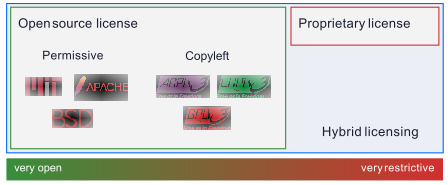
\includegraphics[width=380pt, keepaspectratio]{License_Comparison}
    \caption{License type comparison and examples \parencite{Duras_2020}.}
    \label{fig:license-comparison}
\end{figure}

While the above-mentioned licenses are commonly used to license software, one notable group of licenses commonly applied to other creative works are the \gls{cc} licenses \parencite{Hagedorn_2011}.
These can differ considerably in restrictions they impose on users, from just requiring attribution---\gls{cc} BY\footnote{Available at \url{https://creativecommons.org/licenses/by/4.0/}.}---through disallowing commercial use and mandating the use of the same license---\gls{cc} BY NC SA\footnote{Available at \url{https://creativecommons.org/licenses/by-nc-sa/4.0/}.}---to even prohibiting any adaptation---\gls{cc} BY NC ND\footnote{Available at \url{https://creativecommons.org/licenses/by-nc-nd/4.0/}.} \parencite{Hagedorn_2011}.
As such, they move almost across the whole spectrum of "openness" outlined in Figure~\ref{fig:license-comparison}.
The non-commercial variant is especially controversial as there are differing opinions on what constitutes commercial use \parencite{Hagedorn_2011}.
While for-profit companies using a specific creative work to generate profit are a clear case of commercial use, a work by non-commercial organizations or individuals that is not directly compensated may or may not be classified as commercial use \parencite{Hagedorn_2011}.

\subsubsection{Copyright Exclusions}

In relation to software, there are some aspects that may not constitute a copyrightable work.
A common requirement for work to be copyrightable is for it to be original \parencite{Fisher_2016}.
While the level of originality (creativity) required in the \gls{us} or Japan is considered to be low, within the \gls{eu}, it is higher \parencite{Fisher_2016}.
Under the \gls{eu} law, the work "must reflect the author's own intellectual creation" and the author must be able to make their own choices \parencite[p. 443]{Fisher_2016}.
The latter alludes to external limitations---like when the author has to make certain choices to ensure interoperability \parencite{Fisher_2016}.

Specifically for programming languages, \textcite{Rose_2012} mention the ruling of the \gls{eu}'s highest court that confirmed the "functionality [...] nor the programming language and the format of data files [...] constitute a form of expression [... and so ...] are not protected by copyright [...]" \parencite{cjeu_2012}.
Moreover, it is allowed "to observe, study or test the functioning of that program so as to determine the ideas and principles" \parencite{cjeu_2012}.
It is based on the argument that any other decision would go against the "necessary innovation and competition" \parencite{Rose_2012}.
However, it was made clear this does not apply to the actual source code, object code, or the supplied manual \parencite{Rose_2012}.

Israel's copyright law is thought to be originally largely influenced by British and European law, with recent influences from the more lenient approach of the \gls{us} \parencite{Greenman_2012}.
In relation to software, as is the case in the \gls{eu}, "the idea behind software is not protected by copyright" \parencite{suslina_approaches_2018}.

\subsection{Essential Steps}
\label{sec:oss-essential-steps}

\textcite[Chapter~2]{Fogel_2022} mentions the following as the first steps relevant to this thesis when creating \gls{oss}:

\begin{enumerate}
    \item \textbf{Name}: Choose a name that, among else, can be easily branded, is easy to use even for non-native speakers, and is available as a .com or .org domain.
    \item \textbf{Mission Statement}: Provide a concise description of what the software does so that the user knows "within 30 seconds" \parencite{Fogel_2022} if they are interested.
    \item \textbf{Free}: Make sure to always make it clear the software is free.
    \item \textbf{Features and Requirements}: Make it clear what the software offers and requires.
    \item \textbf{Version Control and Bug Tracking}: Use a publicly accessible place like Github to host the code and manage feature requests and bug reports.
    \item \textbf{Communication}: Provide ways for the users to communicate with the author and between themselves and keep it open and friendly.
    \item \textbf{Guidelines and Documentation}: Offer developer guidelines and (even if short) documentation.
    \item \textbf{Demos}: Show the software works by using videos or images.
\end{enumerate}

When it comes to involving others, \textcite[Chapter~8]{Fogel_2022} suggests keeping in mind most \gls{oss} participants are intrinsically motivated and "credit is the primary currency", should be prevented from "territoriality", and repetitive tasks should be automated as much as possible.
Notably, this includes automated testing, which is important for any modern software project \parencite[Chapter~9]{Sommerville_2019}, but \textcite[Chapter~8]{Fogel_2022} argues it is especially important for \gls{oss}.
Regression tests allow others who are completely unfamiliar---as is often the case with \gls{oss}---to contribute to the code without both authors and contributors fearing breakage.

\subsection{Development and Deployment}

\textcite[Chapter~4]{Sommerville_2019} argues one has to pay attention to the architecture of the software as it has a direct influence on the "performance, usability, security, reliability, and maintainability".
While all of the mentioned aspects are important, each software differs in its needs, and so the prioritisation should follow that \parencite[Chapter~4]{Sommerville_2019}.
Regardless, \textcite[Chapter~4]{Sommerville_2019} mentions the ability to break the application down into smaller meaningful parts (components), which are:

\begin{enumerate}
    \item \textbf{Separated}: Components should have a single purpose.
    \item \textbf{Stable}: Interfaces should be stable and coherent.
    \item \textbf{Unique}: Avoid duplication of the same functionality.
\end{enumerate}

Specifically in relation to the cloud, \textcite[Chapter~5]{Sommerville_2019} argues the main advantages and features one should be looking for are scalability, elasticity, and resilience.
These commonly allow for lower costs, lower time to market, and distribution for users from different parts of the world \parencite[Chapter~5]{Sommerville_2019}.
Some notable considerations when choosing cloud that \textcite[Chapter~5]{Sommerville_2019} mentions include cost, developer experience, privacy and data protection, and portability.
One of the more recent trends is to utilise serverless computing, where the application runs in a completely abstracted away environment with virtually unlimited computing power and a pay-as-you-go pricing model.

In relation to the delivery of the software, \textcites[Chapter~10]{Sommerville_2019}[Chapter~7]{Fogel_2022} concur with the idea the goal is to ship reliable software and to ship often.
DevOps, in particular, is highlighted by \textcite[Chapter~10]{Sommerville_2019} as the preferred modern approach to integration and delivery.
The basic idea is to utilise automation and data to, among else, integrate and deploy the code---\gls{ci} and \gls{cd}.

\subsection{Reliability and Security}

\textcite[Chapter~8]{Sommerville_2019} claims that "high-quality" software not only does what it is expected to do, but is also, among else, reliable, secure, and resilient.
Simple examples of how to achieve reliability offered by \textcite[Chapter~8]{Sommerville_2019} are problem avoidance, input validation, and management of problems.

When it comes to security, the main motivation is to prevent reputation, privacy, or monetary damage done to the users and authors \textcite[Chapter~7]{Sommerville_2019}.
In the case of serverless computing, one significant potential problem is monetary damage from Denial of Service attacks \parencite{Kelly2021}.
Considering the virtually endless scalability and the pay-as-you-go model, instead of endangering availability, the attacks can create an artificial load that can mean significant costs---especially for small projects \parencite{Kelly2021}.

\subsection{Testing}
\label{Literature-Software-Testing}

\textcite[Chapter~9]{Sommerville_2019} maintains code reviews and (automated) software testing are "essential".
While there are many types of testing, the most relevant ones for this thesis are functional---the system does what it should---and user---the system brings value---tests.
The following subsection focuses on functional testing alone as one way of user testing in the form of a comparative study was already covered in detail.

Functional testing involves testing on different levels of abstraction.
The lowest level is testing of the smallest encapsulated parts of the software (units) like functions \parencite[Chapter~9]{Sommerville_2019}.
A level higher in abstraction are feature tests that cover testing the introduced or modified feature \parencite[Chapter~9]{Sommerville_2019}.
The highest level of tests relevant to this thesis are system tests that involve testing the whole product---the combination of its features \parencite[Chapter~9]{Sommerville_2019}.
While lower-level testing is almost always done by developers and is easier to automate, highest level testing is usually done by testers and harder to automate \parencite[Chapter~9]{Sommerville_2019}.
Additionally, experience from the field suggest lower-level tests are more reliable, easier, and cheaper to maintain than higher-level tests \parencites{cohn_succeeding_2010}{Wacker_2015}{Sommerville_2019}.
As such, a common recommendation is to have a higher proportion of unit tests and a lower number of feature and system tests, as illustrated in Figure~\ref{fig:testing-pyramid}.

\begin{figure}[H]
    \centering
    \includesvg[height=200pt, keepaspectratio]{Testing_Pyramid}
    \caption{Testing pyramid originally proposed by \textcite{cohn_succeeding_2010}.}
    \label{fig:testing-pyramid}
\end{figure}

A common question to answer, especially when it comes to unit tests, is how much of the code should be covered.
While at first thought we could argue for the highest possible test coverage, research suggests the relation between the code coverage and benefits like lower number of errors is not linear while the added effort is the highest at very high percentages \parencite{Antinyan2018}.
Looking at a large data set of projects at Google, \textcite{Ivankovic_2019} report an average coverage of a little over 80\%.
